%%%%%%%%%%%%%%%%%%%%%%%%%%
%% Template file for an IEE conference article
%% Trim Size: A4 Paper
%% iiai-conference.tex   :   29-2-08
%% Tex file to use with iiai-c.sty written in Latex2E.
%% The content, structure, format and layout of this style file is the
%% property of International Institute of Applied Informatics
%% Copyright 2013 by International Institute of Applied Informatics
%% All rights are reserved.
%% Created by Satoshi Takahashi, UEC, Japan, Antoine Bossard, AIIT, Japan, Wen Gu, JAIST, Japan and Shun Okuhara, Mie University, Japan
%%%%%%%%%%%%%%%%%%%%%%%%%%
\documentclass[11pt, onecolumn, twoside, a4paper]{article}
\usepackage{iiai-c}
%\usepackage{} % for times new roman; Antoine will send email
%
\usepackage{graphicx}

\usepackage{comment}
\usepackage{amsmath}
\usepackage{amssymb}
\usepackage{amsthm}
\usepackage{lipsum}
\usepackage{mathptmx}


\usepackage[rm,up,sc,topmarks,calcwidth,pagestyles]{titlesec}
\titleformat{\section}{\Large\bfseries\rmfamily}{\thesection}{1em}{}
\titleformat{\subsection}{\large\bfseries\rmfamily}{\thesubsection}{1em}{}
\titleformat{\subsubsection}{\large\it\rmfamily}{\thesubsubsection}{1em}{}

\newtheorem{theorem}{Theorem}
\newtheorem{lemma}[theorem]{Lemma}
\newtheorem{corollary}[theorem]{Corollary}
\newtheorem{property}[theorem]{Property}
\newtheorem{define}[theorem]{Definition}
\newtheorem{assume}[theorem]{Assumption}
\def \Re {\mathbb{R}}


% Edit by IEE editor
\authorshead{S.~Takahashi, A.~Bossard, T.~Matsuo, T.~Fukushima}
\titlehead{IIAI Open Conference Publication Series {\LaTeX} Template}
\vol{1}
\no{1}
\year{2015}
\setcounter{page}{48} % edit
\page{48}
\lastpage{62} % edit


\title{A Platform for Searching Texts for Desired Expressions in a User-editable Pattern Matching Environment for Language Learning}
\author{Tatsuya Katsura \thanks{Graduate School of Environmental, Life, Natural Schience and Technology, Okayama University, Okayama, Japan}, Koichi Takeuchi \thanks{Faculty of Environmental, Life, Natural Science and Technology, Okayama University, Okayama, Japan} }
\date{}
\begin{document} 

\maketitle
\thispagestyle{empty}

\section*{Abstract}
In this paper we propose a platform of pattern matching system that can extract required phrases or sentences in texts.
Finding certain expressions in texts are often needed in language learning, e.g, examples of case markers
between a predicate and an argument, or possible nouns in subject of a verb in a certain meaning. In previous studies,
several types of systems, containing concordancers, are proposed. However, it is not easy to apply combined
patterns because the pattern mathing templates are previously fixed.
% flexibilityが必要 背景としては task specific な systemで作られているので 英語検索に特化はしてると
% 小論文での表現でみんなが同じようにどう使っているかといった表現の分析に利用するのは容易ではない
% その一番の原因は flexibility 
Thus, we propose a flexible phrase searching system in which the users can create search patterns
by combining blocks of basic search templates. % 拡張性がある blockで 提案する
%長すぎる時はここを消す
One of the characteristics the proposed system is that the user can also specify where to be highligted
in texts with the blocks.
To realize the function of combining patterns by the users, the proposed system employs
Prolog as the base of the data structure. The platform of the searching system is implemented
on an Web server with JavaScript-based interface and database system. 
% ブロックにいろいろ設定することで,ユーザは組み合わせてさらに使うことができる
%To realize the pattern matching of predicate-argument structure, 
%the system emplopys several NLP tools.
In the performance test, we shows that the proposed system can deal with relatively large sclale texts
(10,000 sentences), and also demonstrate the combined patterns can be applied to the texts.
In this paper we discuss the system architecture and the extendability of the pattern matching. 
%
%\section*{Keywords}
%About four key words or phrases in alphabetical order, separated by commas.
%
%\noindent
\\[2mm]
{\it Keywords: } Pattern matching, Concordancer, Block-based programming, Prolog


\section{Introduction}
%education
Extraction of some phrases and expressions in texts is considered essential function in langugage education.
For example, case markers located between a predicate and an object in Japanese language are various
rules and alternations\footnote{The verbs {\it morau} (get) and {\it eru} (obtain) are almost the same meaning
but {\it morau} has alternation between the case markers {\it ni/kara} as {\it kare ni/kara morau}
((I) get (it) from him.), and 
{\it eru} can only takes {\it kara} in this meaning as {\it kare kara/*ni eru}.},
% 彼 から もらう,彼に もらう but, 彼から 得る 彼に 得る.
then language learners need to search for examples of predicate-argument
examples in Japanese texts. 
%also, search for similar phrases in student essays. this is eample for use in education. 
As a tool for searching texts, various kinds of concordancer are proposed, however, most concordancers
are targeted for English. From the results of natural language processing study, several dependency parsers for
Japanese are available, thus it is possible to compose a complex text searching system if
the language learners can build NLP tools. But language learners are not NLP or software engineer,
thus, we need an environment to build patterns by searching for phrases or expressions without
needing programming.


when user want to obtain some verb-nouns or predicate preposition,
concodancer is available the basic functions character, word matchina are available,
but more extendede cases are no method. 

, however, more combined search, for example, semantic meaning
of predicate buy-sell and linguitic alternation, kara/wo in Japanese
dependency 

% もらう,得るの質問 native https://ja.hinative.com/questions/17482159





%作ったもの
日本語に対するパターンマッチングシステム



\section{Related Studies}
An IIAI electronic copyright form should accompany your final submission or registration of the conference. The instruction of copyright transfer is announced at the conference webpage. Authors are responsible for obtaining any security clearances for the copyright form submission.


\section{Platfrom of Pattern Matching System}
user editable pattern with visual handling, Construction of pattern is not easy, the
user shoud apply the assumed patterns, see the results and then tune up the patterns.
Thus, editing space and results should be exist.

Patterns are combinations, conbining by basic blocks and extract every where matched.




\section{既存の言語パターンマッチシステムの概要と改善点}




%本章では既存のパターンマッチシステムの全体像と,改善が必要な問題点について述べ
%る.2.1節で既存のパターンマッチシステムの全体像について述べ,2.2節に既存のシステムの問題点を挙げ,2.3節では2.2節で挙げた問題点に対する改善案について説明をする.

This chapter describes the overall picture of the existing pattern matching system and the problems that need to be improved. Section 2.1 describes the overall picture of the existing pattern matching system, Section 2.2 lists problems with the existing system, and Section 2.3 describes proposed improvements to the problems listed in Section 2.2.


\subsection{既存の言語パターンマッチシステムの全体像}

%本節では既存のパターンマッチシステムの全体像について説明する.既存のパターンマッチシステムを図\ref{figure:1}
%に示す.
%既存のパターンマッチシステムは情報を抽出したいテキスト文を解析し,その解析結果から,ユーザ自らが対象に予め関係する文や文の一部に対応する文構造のパターンを用意し,パターンに合致する結果を取得するというものである.実際の処理の流れは図\ref{figure:2}に記載してある.

This section describes the overall picture of the existing pattern matching system. The existing pattern-matching system is shown in Figure 1.
Figure 1 shows the existing pattern matching system.
Existing pattern matching systems analyze text sentences from which information is to be extracted, and from the analysis results, users prepare patterns of sentence structures corresponding to sentences or parts of sentences related to the target in advance, and obtain results that match the patterns. The actual flow of the process is shown in Figure%\ref{figure:2}.
\begin{figure}[htbp]
\centering
%\includegraphics[width=100mm]{figure1.png}
\caption{既存のパターンマッチシステムの構成図}
\label{figure:1}
\end{figure}
\begin{figure}[htbp]
\centering
%\includegraphics[width=100mm,scale=0.5]{figure2.png}
\caption{既存のパターンマッチシステムの処理の流れ}
\label{figure:2}
\end{figure}
%既存のシステムはユーザが実際に操作するフロントエンドと,フロントエンドから受け取ったデータを処理するバックエンドで構成される.その詳細を以下の\ref{sec:2-1-1}節,\ref{sec:2-1-2}節で説明する.
Existing system is a front that the user actually operates. The system consists of a front end and a back end that processes data received from the front end.
The details are described in sections 2.1.1 and 2.1.2 below.

\subsubsection{フロントエンド}
\label{sec:2-1-1}
%フロントエンドは主にJavaScriptのフレームワークReactを用いて構築しており,以下のような機能を有している.
The frontend is mainly built using the JavaScript framework React, and has the following functions.

\begin{description}
   \item[コーパスアップロード]\mbox{}\\
%解析対象のコーパスファイルのアップロードを行う.文の区切りは句点,感嘆符お
%よび疑問符で認識される.
Upload the corpus file to be analyzed. Sentence breaks are recognized by punctuation marks, exclamation points
and question marks.
   \item[コーパス解析結果表示]\mbox{}\\
%以下の図\ref{corpus_results}のようなコーパスの解析結果を表示する.
\begin{comment}
\begin{figure}[htbp]
 \begin{minipage}[b]{0.45\linewidth}
    \centering
    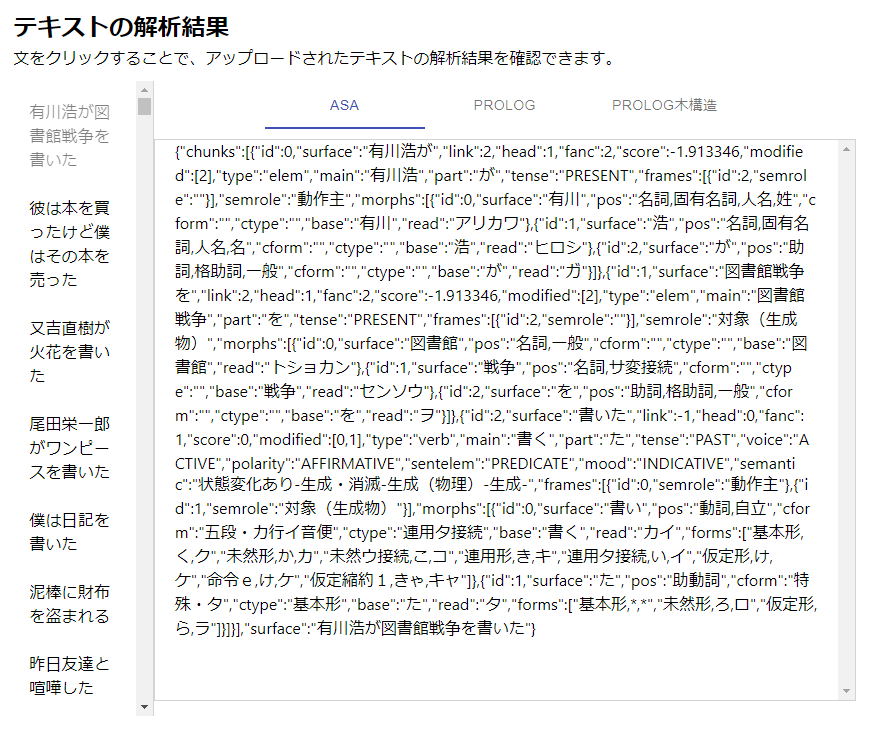
\includegraphics[keepaspectratio, scale=0.4]{figure/asa_results.png}
  \subcaption{ASA}\label{figure:3-1}
  \end{minipage}
  \begin{minipage}[b]{0.45\linewidth}
    \centering
    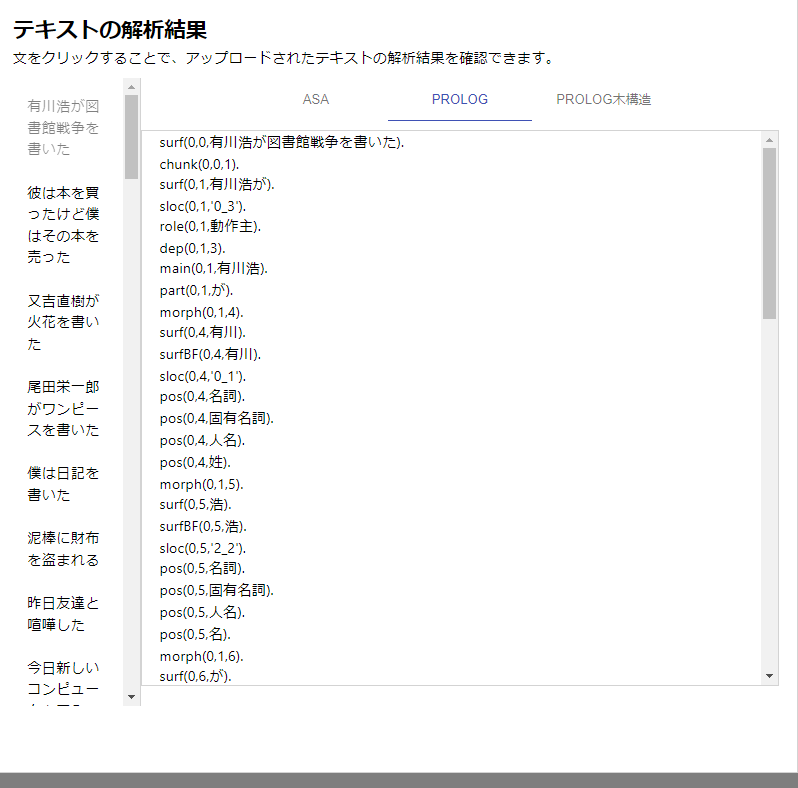
\includegraphics[keepaspectratio, scale=0.4]{figure/prolog.png}
    \subcaption{Prolog}\label{figure:3-1}
  \end{minipage}
  \begin{minipage}[b]{0.45\linewidth}
    \centering
    \includegraphics[keepaspectratio, scale=0.4]{figure/prolog木.png}
    \subcaption{木構造}\label{figure:3-2}
  \end{minipage}
  \caption{解析結果の表示}\label{corpus_results}
\end{figure}
\end{comment}

\item[言語パターン構築]\mbox{}\\
%Blocklyを用いて視覚的にブロックを組み合わせることで検索したい言語パターンを構築することがで
%きる.多種のブロックを組み合わせることにより,ASAの解析結果の情報を複雑に
%検索することができる.図\ref{blockly:1}は著者と作品を抽出する言語パターンである.
Using Blockly, you can construct the language pattern you want to search for by visually combining blocks.
By combining many different types of blocks, the information in the ASA analysis results can be complex. By combining many different types of blocks, it is possible to search for information on ASA parsing results in complex ways.
Figure 1. Figure is a language pattern for extracting authors and works.

\begin{comment}
\begin{figure}[htbp]
  \centering
  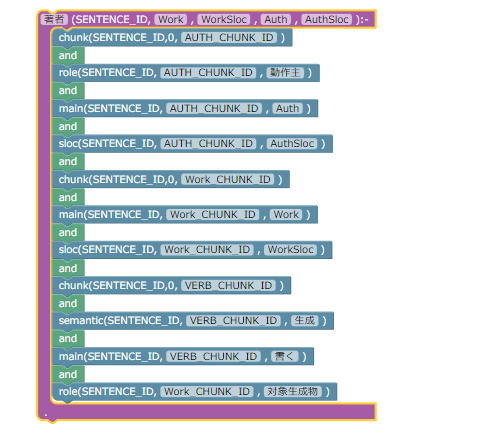
\includegraphics[scale=.3]{figure/make_pattern.png}
  \caption{Blocklyによる「著者」と「作品」を抽出する言語パターン}
  %\label{blockly}
\end{figure}
\end{comment}

%また構築した言語パターンを xml 形式のファイルにエクスポートすることができる.エク
%スポートしたファイルをインポートすることもできる.
It is also possible to export the constructed language patterns to xml format files.
The exported file can also be imported.
\item[言語パターンマッチ結果表示]\mbox{}\\
%言語パターンマッチの実行結果を表示する.表示形式には,KWIC 形式,強調形式,
%テーブル形式がある.図\ref{blockly:1}の言語パターンを検索クエリとして言語パターンマッチを実行した結果が図\ref{display_result}である.AuthSlockは作品,WorkSlocは著者を意味しており,それぞれの形式でコンコーダンス表示されている.
Displays the results of language pattern matching. The display format includes KWIC format, highlighting format, and
table format. Figure  shows the result of executing language pattern matching using the language pattern in Figure 

\begin{comment}
\begin{figure}[htbp]
 \begin{minipage}[b]{0.45\linewidth}
    \centering
    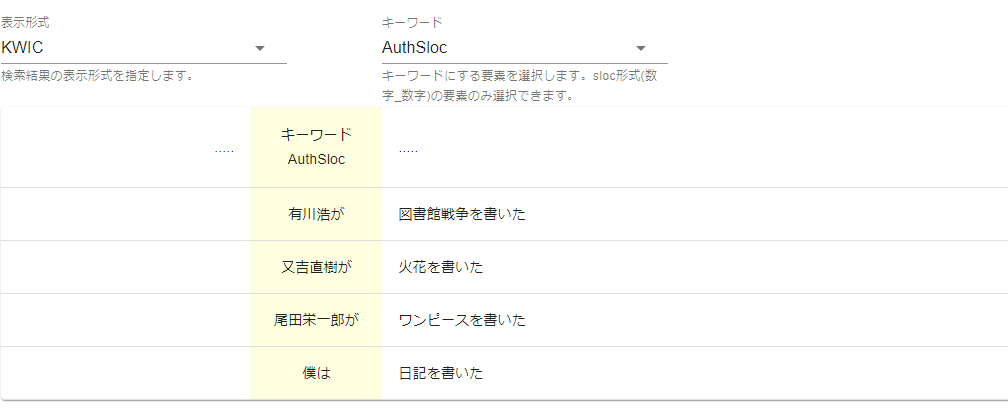
\includegraphics[keepaspectratio, scale=0.4]{figure/KWIC_results.png}
    \subcaption{KWIC}\label{figure:KWIC}
  \end{minipage}
  \begin{minipage}[b]{0.45\linewidth}
    \centering
    \includegraphics[keepaspectratio, scale=0.4]{figure/csent_results.png}
    \subcaption{強調}\label{figure:acsent}
  \end{minipage}
  \begin{minipage}[b]{0.45\linewidth}
    \centering
    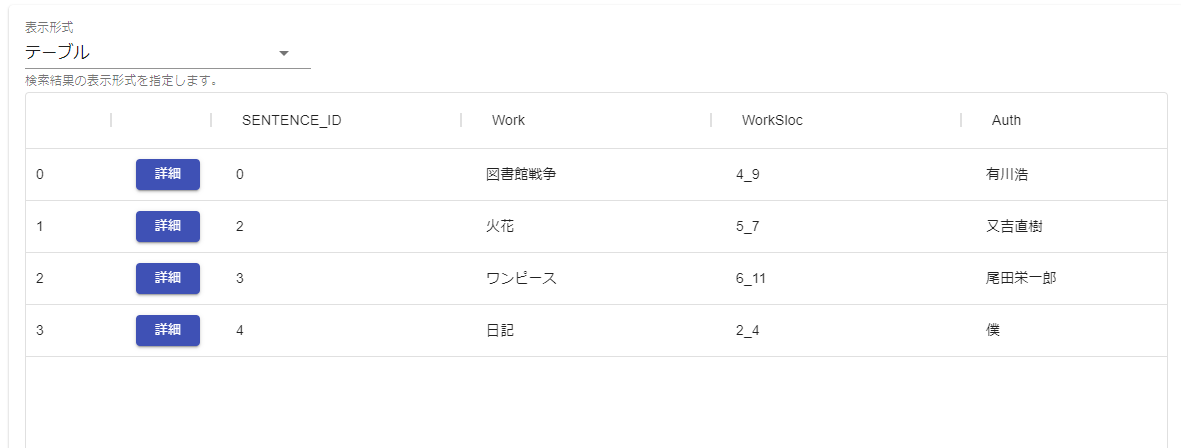
\includegraphics[keepaspectratio, scale=0.4]{figure/table_results.png}
    \subcaption{テーブル}\label{figure:table}
  \end{minipage}
  \caption{言語パターンマッチ結果表示}\label{display_result}
\end{figure}
\end{comment}
\end{description}





\subsubsection{バックエンド}
%バックエンドはPython Web フレームワークである Djangoで構築されている. ASAによる解析にはasapy, Prolog処理系にはprologpyを用いて実装されている.
The backend is built on Django, a Python web framework. It is implemented using asapy for analysis by ASA and prologpy for Prolog processing.

\label{sec:2-1-2}
\begin{description}
\item[コーパス解析]\mbox{}\\
%解析対象のコーパスを読み込み,ASA による解析, Prolog への変換を行う.
%生成した解析結果をフロントエンドに返却し,ブラウザのメモリに保存する.
Reads the corpus to be parsed, parses it with ASA, and converts it to Prolog.
The generated analysis results are returned to the front end and stored in the browser's memory.
\item[言語パターンマッチ]\mbox{}\\
%対象の Prolog と検索クエリに対し,Prolog 処理系によるクエリ検索を行う.
%生成したパターンマッチ結果をフロントエンドに返却し,ブラウザのメモリに保存する.
Query the target Prolog and search query using the Prolog processor.
The generated pattern matching results are returned to the front end and stored in the browser memory.
\end{description}


%%%コメントアウト%%%%%
\begin{comment}
\subsection{既存のシステムの問題点}
\label{sec:2-2}
本節では,既存のパターンマッチシステムの問題点について大きく2つ説明する.

一つ目の問題としては英語を含んだ文のパターンマッチができないことである.現在のパターンマッチで利用しているProlog処理系はPythonで作成した簡易版であるため,ANDやORなどの英語の論理演算子のような特定の単語の入力を受け付けないからである.将来的に複雑なテキストを処理する際にボトルネックとなるため,このような問題を解決するための別の処理系の実装が求められる.

二つ目の問題としては大規模のコーパスの入力を受け付けないことである.現在のパターンマッチシステムでは1度に解析できる文数に限度があり,1000文のテキストを解析することでさえ約20分以上かかり,5000 文以上のテキストをアップロードして解析しようとすると動作が止まってしまう.
現在のシステムでは,解析結果返却の際に,テキストデータをブラウザのメモリに保存しているため.大規模なコーパスの入力を受け付けない.またその言語パターンマッチをバックエンド側で行う際にテキストデータを再送信しているためフロントエンドとバックエンドの通信する回数やデータ量が多くなってしまうため,動作時間が増加している.このような問題を解決するためにデータベースを導入するなどテキストデータの保存先の変更することにより,大規模なテキストコーパスでも解析およびパターンマッチで動作可能にし,動作時間をさらに向上することが求められる.
\subsection{言語パターンマッチシステムの改善点の整理}
\label{sec2-3}
本節では,既存のパターンマッチシステムの改善案について整理する.\ref{sec:2-2}節の問題を受け,以下のような改良案が挙げられる.以降の章で詳細を述べる.
\begin{itemize}
\item 既存のProlog処理系をSWI-Prologに変更する
\item データベースとしてElasticsearchを導入する

\end{itemize}
\end{comment}

%\begin{figure}[htbp]
% \begin{center}
%    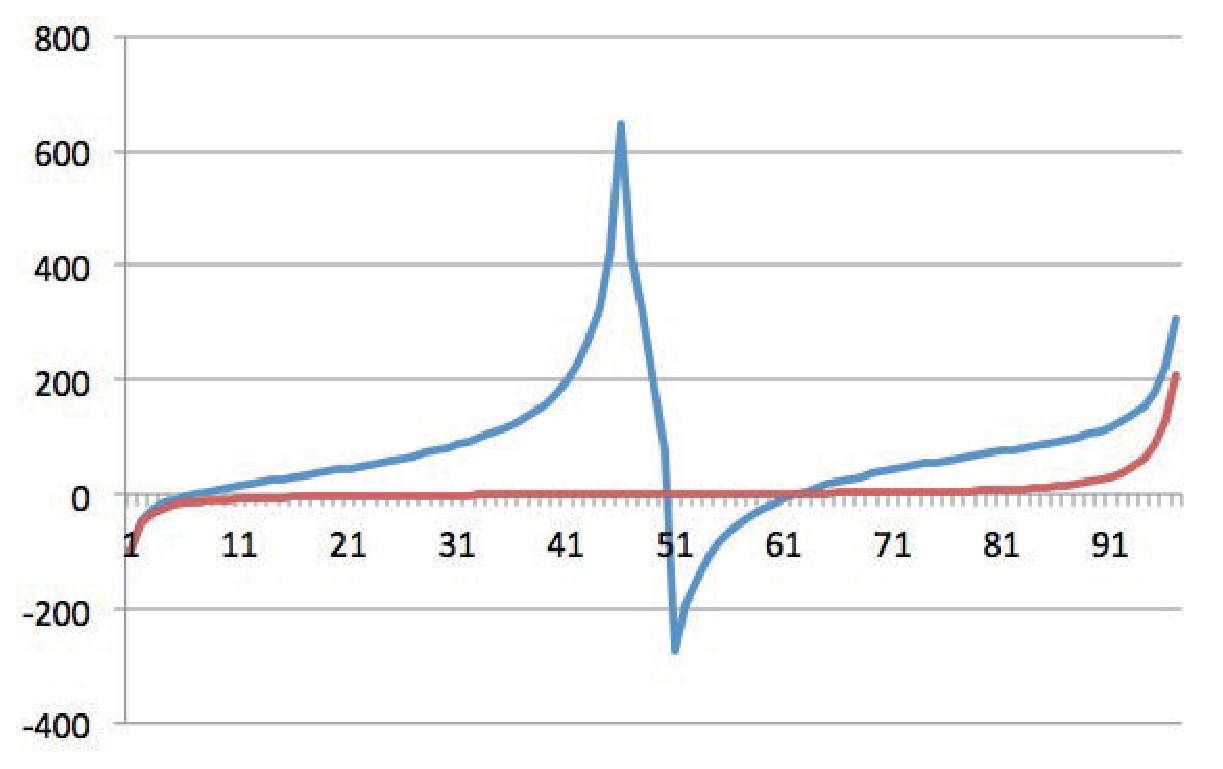
\includegraphics[clip,width=10.0cm]{./fig1.eps}
%    \caption{Example}
%    \label{fig:example}
%  \end{center}
%\end{figure}


\section{References}


\subsection{Example}
\subsubsection{Article in a collection}
\subsubsection{Article in a conference proceedings}
\subsubsection{Article in a journal or magazine}
\subsubsection{Blog}
\subsubsection{Book}
\subsubsection{Book series}
\subsubsection{Electronic publication(Article in a conference proceedings)}
\subsubsection{Electronic publication(Online-only publication)}
\subsection{Abbreviations in References}

%\begin{table}[hbtp]
% \caption{Abbreviations}
% \label{table:data_type}
% \begin{center}
%  \begin{tabular}{ll}
%   \hline
%   Abbreviations & Word  \\
%   \hline \hline
%Conf. & Conference (on)\\
%Vol. & Volume\\
%   \hline
%  \end{tabular}
% \end{center}
%\end{table}




\section{Some Common Mistakes}



\section*{Acknowledgments}

Author can include an acknowledgement of this work here. 


\begin{thebibliography}{9}
\bibliographystyle{unsrt_abbrv}
\bibitem{11} Consolidating the IT Infrastructure, white paper, Oracle Corp., Dec. 2003.
\end{thebibliography}
\end{document}